\documentclass{article}

\usepackage{amsmath}
\usepackage{amsthm}
\usepackage{amsfonts}
\usepackage{framed}

% For including other sections 
\usepackage{standalone}

%% Simple AMSthm environments, numbered together.
\newtheorem{lem}{Lemma}
\newtheorem{thm}[lem]{Theorem}
\newtheorem{conj}[lem]{Conjecture}

\theoremstyle{definition}
\newtheorem{defn}[lem]{Definition}

% Various mathematical helper definitions
\newcommand{\Z}{\mathbb{Z}}



\title{Project 2 Report}
\begin{document}
\maketitle

\section{Overview}
\begin{framed}
  Discuss the high level goals of your work, along with any
  interesting/key findings.
\end{framed}

Our objective was to understand and experience the issues that arise
when actually implementing program analyses. To this end, we
constructed a dataflow analysis framework based on the LLVM compiler
infastructure.

We confirmed through experience that SSA makes flow functions
\emph{much} easier to write. We found that the most helpful part of
the LLVM API is the object hierarchy for dealing with the graph of
Value objects representing LLVM IR. Subclasses of Value are rich,
representing functions, basic blocks, instructions, constants,
etc. These IR object classes provide many useful convienence functions
and make it easy to traverse the program. The least helpful parts of
the LLVM API is the pass manager and the special LLVM replacement for
C++ run-time type information; these features are obscure and
difficult to use.

The most surprising feature of LLVM was the InstVisitor template
class. This class made our implementation much easier and cleaner than
it would have been otherwise, but examples in the introductory
documentation do not use it. For something so helpful to LLVM
newcomers, InstVisitor is poorly advertised in the LLVM documentation.

Though the analyses were relatively straightforward in terms of flow
functions, the technical hurdles of actually making them work were
nontrivial, and we learned a great deal. This project provided a solid
foundation of practical experience for building programming-language
tools based on LLVM. We document our implementation efforts in the
following pages, beginning with the overall design for the dataflow
analysis framework. 

% We found numerous conceptual mismatches between the LLVM IR and other
% programming languages (including assemblers). Registers may only be
% assigned to at one site of the program (SSA), and variables in a
% high-level language may be represented by either a sequence of these
% registers or as a memory location. The expressions of a high-level
% language can become chains of instructions in the IR, changing the
% definition of CSE. The reasons for these design choices became clear
% as we worked our way through implementation of the analyses, and will
% be expanded on in the appropriate sections.


\section{Interface Design}
\begin{framed}
  Describe interface. Discuss what alternative designs you may have
  also considered, and explain the tradeoffs that ultimately led to
  your choice.
\end{framed}


\begin{description}
\item[LatticePoint] Every dataflow analysis requires a Lattice to work
  over. The \emph{LatticePoint} class describes our interface to these
  points. Anything that inherits from \emph{LatticePoint} must
  implement:
  \begin{description}
  \item[equals$(LP) \rightarrow $Bool] Compare this latticepoint and
    the argument for equality, returning a Boolean.
  \item[join$(LP) \rightarrow LP$] Return a new LatticePoint
    containing the join of this LatticePoint and the argument.
  \item[isBottom$() \rightarrow $Bool] Returns true if this
    latticePoint is Bottom
  \item[isTop$() \rightarrow $Bool] Returns true if this latticePoint
    is Top.
  \end{description}
\item[FlowFunction] This class provides an interface to calling flow
  functions. Derived classes must implement a single special function:
  \[
  \textbf{operator}(Instruction, Vector \langle LP\rangle) \rightarrow
  Vector \langle LP \rangle
  \]
  Implementing the ``operator'' function makes objects of this type
  callable. To define each analysis we make a subclass of
  \emph{FlowFunction} that can operate on a particular type of
  \emph{LatticePoint}. When ``operator'' is called, a single step of
  the flow function is exectued with the argument \emph{LatticePoints}
  as incoming edges on the control flow graph. A vector of
  \emph{LatticePoints} that should be on the outgoing edges of this
  instruction is returned.
\item[Analysis] This class contains the implementation of the worklist
  algorithm. It is not an interface, and is not meant to be derived
  from. It has one public function:
  \[
  \textbf{analyze}(Function, FlowFunction, LP) \rightarrow
  Map \langle Instruction, LP \rangle
  \]
\end{description}

To use our framework, a caller  first instanciates a ``bottom''
\emph{LatticePoint} and a \emph{FlowFunction} of matching types. Then,
in an LLVM Pass, the caller supplies a function and the aforementioned
objects to \textbf{analyze}. 

Adding an additional analysis to the framework amounts to providing
new derived classes of \emph{LatticePoint} and \emph{FlowFunction}.

% issue with this design: positional encoding of true/false branches
% (or whatever) in the return type of operator()

Unsure how honest to be here. Tradeoffs ended up being, how many C++
features can we avoid and still have a functioning C++ program? Other
than this issue, describing our interface (flowfunction object,
latticepoint object, and a blob of code implementing the worklist
algorithm that uses runtime polymorphism to use these objects) is
pretty straightforward. I (marco) can write this.

\section{Analyses}

\subsection{Constant Propagation}
\documentclass{article}

\usepackage{amsmath}
\usepackage{amsthm}
\usepackage{amsfonts}
\usepackage{framed}

%% Simple AMSthm environments, numbered together.
\newtheorem{lem}{Lemma}
\newtheorem{thm}[lem]{Theorem}
\newtheorem{conj}[lem]{Conjecture}

\theoremstyle{definition}
\newtheorem{defn}[lem]{Definition}

\begin{document}

\subsubsection{Mathematical Flow Functions}

The constant propagation analysis is a `must' analysis. Thus, we define the lattice to be $(D, \sqsubseteq, \top, \perp, \sqcup, \sqcap)$ = $(2^A, \supseteq, A, \emptyset, \cap, \cup)$ where

\[ A = \{x \rightarrow N~|~x \in \textup{Vars} \wedge x \in \mathbb{Z}\} \].

The flow functions implemented in our framework are as follows:

\[ F_{X:= Y \text{op} Z}(in) = in - \{X \rightarrow \ast\} \cup \{ X \rightarrow N~|~(Y \rightarrow N_1) \in in~\wedge ~(Z \rightarrow N_2) \in in~\wedge ~N = N_1~op~N_2 \} \]

\[ F_{if(X == C) \text{true-branch}}(in) = in - \{X \rightarrow \ast\} \cup \{ X \rightarrow C \} \]

\[ F_{if(X != C) \text{false-branch}}(in) = in - \{X \rightarrow \ast\} \cup \{ X \rightarrow C \} \]

At a join (i.e. PHI node), we take the intersection between the two incoming lattice points.

\[ F_{\text{merge}}(in_1, in_2) = in_1 \sqcup in_2 \]

\subsubsection{Implementation Considerations}

Our design simply handles constant propagation by storing mappings of Value* to ConstantInt*. Because using mem2reg does constant folding already, the flow functions are limited to simply performing binary operations, propagating constants in branches when we check for equality and inequality, and handling PHI nodes.

Binary operations are fairly straight forward. Since we know the value of the constants at compile time, we can evaluate them and propagate. For branching instructions, we know that if a statement such as \verb|if(x == 9)| evaluates to true, then \verb|x| has the value 9 in that branch. Similarly, if we have the statement \verb|if(x != 9)|, then we know the false branch can map \verb|x| to 9. Finally, at PHI nodes, we can simply find the intersection of two branches.

\end{document}



\subsection{Available Expressions}
\documentclass{article}

\usepackage{amsmath}
\usepackage{amsthm}
\usepackage{amsfonts}
\usepackage{framed}

%% Simple AMSthm environments, numbered together.
\newtheorem{lem}{Lemma}
\newtheorem{thm}[lem]{Theorem}
\newtheorem{conj}[lem]{Conjecture}

\theoremstyle{definition}
\newtheorem{defn}[lem]{Definition}

\begin{document}

\subsubsection{Mathematical Flow Functions}
The available expressions analysis is a ``must'' analysis. Thus, we
define the lattice to be $(D, \sqsubseteq, \top, \perp, \sqcup,
\sqcap)$ = $(2^A, \supseteq, A, \emptyset, \cap, \cup)$ where

\[ A = \{x \rightarrow N~|~x \in \textup{Values} \wedge x \in \textup{Instructions}\} \].

Values and instructions are the LLVM types corrosponding to Value
pointers and instruction pointers, respectively. The idea is that
instructions are the set of expressions in LLVM.

The flow functions implemented in our framework are as follows.

\begin{center}
\begin{tabular}{c | c} % centered columns (4 columns) 
Function & Output \\ [0.5ex] % inserts table 
%heading 
\hline % inserts single horizontal line 
$F_{X:= Y \text{op} Z}(in)$ & $in \cup \{ X \rightarrow W : \exists \langle W, E\rangle \in in.  E = Y \text{op} Z\} \cup$ \\
& $\{ X \rightarrow Y \text{op} Z : \neg\exists \langle W, E\rangle \in in.  E = Y \text{op} Z\}$\\
$F_{if(*) \text{true-branch}}(in)$ & $in$ \\ 
$F_{if(*) \text{false-branch}}(in)$ & $in$ \\ 
$F_{X := \varphi(Y,Z)}(in_1, in_2)$ & $(in_1 \cap in_2) \cup \{X \rightarrow E : \langle Y, E \rangle \in in_1 \wedge \langle Z,E \rangle \in in_2 \}$\\
$F_{X := \text{cmp}(Z,Y)}(in)$ & $in$\\
 [1ex] % [1ex] adds vertical space 
\hline %inserts single line 
\end{tabular} 
\end{center}
\subsubsection{Implementation Considerations}
Most of the implementation of available expression analysis flow
functions was straightforward. There were, for example, no issues with
potentially infinite sets because each program is a fintie set of
expressions. The data structures used were simple
\texttt{std::maps}. 

The most involved thing we implemented was correctly deciding
$\varphi$ nodes that have arbitrary numbers of arguments, not just a
pair of arguments. This is not represented in the mathematical
flowfunction above (the notation was too cumbersome), but our
implementation handles $n$-ary $\varphi$ nodes by overlapping pairwise
comparisons of all operands. 

The most challenging aspect of this implementation would have been
comparing distinct instructions to see whether they are semantically
equal or not. Our implementation does the easiest thing possible,
which is calling the member function of the Instruction class
\texttt{isIdenticalToWhenDefined}. Unfortunately, this member function
only decides syntactic equivalence. So, for example, a commutative
operator like \texttt{add} will not compare equal if the operands are
in the wrong order.

If we had more time, we would have added some extra intelligence to
the equivalence test. For example, for commutative operators it would
be conceptually simple to swap operands into lexicographic order by
pointer and then compare.

\end{document}



\subsection{Range Analysis}
\documentclass{article}

\usepackage{amsmath}
\usepackage{amsthm}
\usepackage{amsfonts}
\usepackage{framed}

%% Simple AMSthm environments, numbered together.
\newtheorem{lem}{Lemma}
\newtheorem{thm}[lem]{Theorem}
\newtheorem{conj}[lem]{Conjecture}

\theoremstyle{definition}
\newtheorem{defn}[lem]{Definition}

\begin{document}

\subsubsection{Mathematical Flow Functions}

\begin{framed}
  define your lattice and flow functions in mathematical notation
  (i.e., in the style used in the lecture notes and on the midterm).
\end{framed}

Unlike the previous two analyses, range analysis is a `may' analysis. Thus the most conservative range for a variable is the full set and the most optimistic is the empty set. With these considerations in mind, let us define our lattice and flow functions. 

One may be tempted to write the domain as

\[ 2^{ \{ x \rightarrow [a , b] \; | \; x \in \text{Vars} \, \wedge \, -\infty \leq a \leq b \leq \infty \} }.  \]

While this has the correct intuition, it is quite imprecise, as we do not want there to be the possibility of a variable having more than one range. Given a variable $x \in$ Vars, let us define $D_x$ as the domain of $x$, i.e. 

\[ D_x =  2^{ \{ x \rightarrow [a , b] \; | \;  -\infty \leq a \leq b \leq \infty \} }. \]

Then our final domain is the Cartesian product of $D_x$'s, which we write as

\[ D = \prod_{x \in \text{Vars}} D_x. \]

Top will correspond to the product of full sets, that is if $x_1, x_2, \ldots$ is an enumeration of Vars, then

\[  \top = (x_1 \rightarrow [-\infty, \infty], x_2 \rightarrow [-\infty, \infty], \ldots). \]

Similarly, we have

\[ \bot =  (x_1 \rightarrow \emptyset , x_2 \rightarrow \emptyset, \ldots). \]

Given two elements of our domain, $A, B \in D$, we can write $A = (x_1 \rightarrow [a_1, b_1] , x_2 \rightarrow [a_2, b_2], \ldots)$ and $B = (x_1 \rightarrow [a'_1, b'_1] , x_2 \rightarrow [a'_2, b'_2], \ldots)$. Then $A \sqsubseteq B$ if and only if $[a_i, b_]) \subseteq [a'_i, b'_i]$ for all $i$. Additionally, if for all $i$, we let $\overline{a_i} = \max \{ a_i, a'_i \}$ and $\underline{a_i} = \min \{ a_i, a'_i \}$ (similarly for $\overline{b_i}$ and $\underline{b_i})$, then we can write

\[ A \sqcup B = (x_1 \rightarrow [\underline{a_i}, \overline{b_1} ], x_2 \rightarrow [\underline{a_2}, \overline{b_2} ] )\]

\noindent and

\[ A \sqcap B = (x_1 \rightarrow [\overline{a_i}, \underline{b_1} ], x_2 \rightarrow [\overline{a_2}, \underline{b_2} ] )\]

\noindent where we take the convention that $[a, b] = \emptyset$ if and only if $b < a$. Now that the lattice has been defined, let's turn our attention to the various flow functions. To make the analysis more concrete, given an element $A \in D$ where let $A(x_i \rightarrow [a', b'])$ denote the exact same element of $D$ with the exception that the new range of $x_i$ is $[a', b']$.



\subsubsection{Implementation Considerations}
\begin{framed}
  discuss how you actually went about implementing the lattice and
  flow functions. For instance, some interesting questions are: what
  data structure(s) did you use, and how do you represent potentially
  infinite sets? How are input facts passed to your flow functions,
  and how do output facts get propagated?
\end{framed}

\end{document}




\subsection{Intra-Procedural Pointer Analysis}
\documentclass{article}

\usepackage{amsmath}
\usepackage{amsthm}
\usepackage{amsfonts}
\usepackage{framed}

%% Simple AMSthm environments, numbered together.
\newtheorem{lem}{Lemma}
\newtheorem{thm}[lem]{Theorem}
\newtheorem{conj}[lem]{Conjecture}

\theoremstyle{definition}
\newtheorem{defn}[lem]{Definition}

\begin{document}

\subsubsection{Mathematical Flow Functions}
Like range analysis, pointer analysis is a `may' analysis. The domain of the analysis can be written as

\[ D = 2^{\{ x \rightarrow y \; |  \; x \in \text{Vars} \, \wedge \, y \in \text{Vars} \}}. \]

Top and bottom are the full set and the empty set, respectively. Thus, $top =\{ x \rightarrow y \; |  \; x \in \text{Vars} \, \wedge \, y \in \text{Vars} \}  $ and $\bot = \emptyset.$ Finally, we have $\sqsubseteq \, = \, \subseteq$, $\sqcup = \cup$, and $\sqcap = \cap$. The flow functions for pointer analysis can be written as follows

\begin{center}
\begin{tabular}{c | c} % centered columns (4 columns) 
Function & Output \\ [0.5ex] % inserts table 
%heading 
\hline % inserts single horizontal line 
$F_{X = C}(in)$ & $in \setminus \{ X \rightarrow * \}$ \\ % inserting body of the table 
$F_{X = Y + Z}(in)$ & $in \setminus \{ X \rightarrow * \}$ \\ 
$F_{X = Y}(in)$ & $in \setminus \{ X \rightarrow * \} \cup \{ X \rightarrow Z \, | \, Y \rightarrow Z \in in \}$ \\ 
$F_{X =  \& Y}(in)$ & $in \setminus \{ X \rightarrow * \} \cup \{ X \rightarrow Y \}$\\ 
$F_{X = *Y}(in)$ & $in \setminus \{ X \rightarrow * \} \cup \{ X \rightarrow B \; | \; \exists A \in \text{Vars s.t. }  Y \rightarrow A \in in \, \wedge \, A \rightarrow B \in in \}$\\
$F_{*X = Y}(in)$ & $in \setminus \{ X \rightarrow * \} \cup \{ A \rightarrow B \; | \; \exists B \in \text{Vars s.t. } X \rightarrow A \in in \, \wedge \, Y \rightarrow B \in in\}$\\ [1ex] % [1ex] adds vertical space 
\hline %inserts single line 
\end{tabular} 
\end{center}

%\[ F_{X = C}(in) = in \setminus \{ X \rightarrow * \} \]
%
%\[ F_{X = Y + Z}(in) = in \setminus \{ X \rightarrow * \} \]
%
%\[ F_{X = Y}(in) = in \setminus \{ X \rightarrow * \} \cup \{ X \rightarrow Z \, | \, Y \rightarrow Z \in in \}\]
%
%\[ F_{X =  \& Y}(in) = in \setminus \{ X \rightarrow * \} \cup \{ X \rightarrow Y \}\]
%
%\[ F_{X = *Y}(in) = in \setminus \{ X \rightarrow * \} \cup \{ X \rightarrow B \; | \; \exists A \in \text{Vars s.t. }  Y \rightarrow A \in in \, \wedge \, A \rightarrow B \in in \}\]
%
%\[ F_{*X = Y}(in) = in \setminus \{ X \rightarrow * \} \cup \{ A \rightarrow B \; | \; \exists B \in \text{Vars s.t. } X \rightarrow A \in in \, \wedge \, Y \rightarrow B \in in\}\]


\subsubsection{Implementation Considerations}
\begin{framed}
  discuss how you actually went about implementing the lattice and
  flow functions. For instance, some interesting questions are: what
  data structure(s) did you use, and how do you represent potentially
  infinite sets? How are input facts passed to your flow functions,
  and how do output facts get propagated?
\end{framed}

\end{document}




\section{Testing}

\documentclass{article}

\usepackage{amsmath}
\usepackage{amsthm}
\usepackage{amsfonts}
\usepackage{framed}

%% Simple AMSthm environments, numbered together.
\newtheorem{lem}{Lemma}
\newtheorem{thm}[lem]{Theorem}
\newtheorem{conj}[lem]{Conjecture}

\theoremstyle{definition}
\newtheorem{defn}[lem]{Definition}

\begin{document}

\begin{framed}
  Make sure to explain assumptions you make about the code you
  analyze. For instance, for pointer analysis, you may have made some
  assumptions about the aliasing information known about input
  parameters. Explain those assumptions and why they are reasonable.

  Part of this project is to come up with a useful set of benchmarks
  on which to test and improve your analysis. Discuss why you chose
  those benchmarks, and what makes them interesting. If your
  implementation fails on some benchmarks (there's no shame in it!),
  then explain why and how the analysis might be improved.
\end{framed}

The difficulty of getting the various analyses to work properly on a
piece of code is tightly coupled with the complexity of the underlying
control flow graph. Pathologies that underly implementations of flow
functions may not arise in straight-line programs but become painfully
obvious when branches are introduced. Our benchmarks are designed to
illustrate that our analyses are robust to non-trivial control flow
structures.

Broadly speaking, we have three types of benchmark. The first type is
straight-line programs, which introduce no branches in control
structure. They are the easiest to handle, and our analyses are
accordingly precise on them. Simple branching programs are the second
type, and they introduce conditional branches into fold, but do not
exhibit loops. They are slightly more challenging, but SSA makes them
much easier to handle. Our final type of benchmark is looping
programs. As their name suggests, they have loops, which makes
precision quite difficult.

\subsection{Benchmarks/Assumptions in Common}
Because we have a common pool of benchmarks, we can list them here
along with common assumptions on code. More specialized discussion of
per-analysis benchmark goes below. Here, we can also introduce the
Straight Line Program/Branching Program distinction.

\subsection{Constant Propagation}
\subsection{Available Expressions}
A straight line program where we can do CSE:
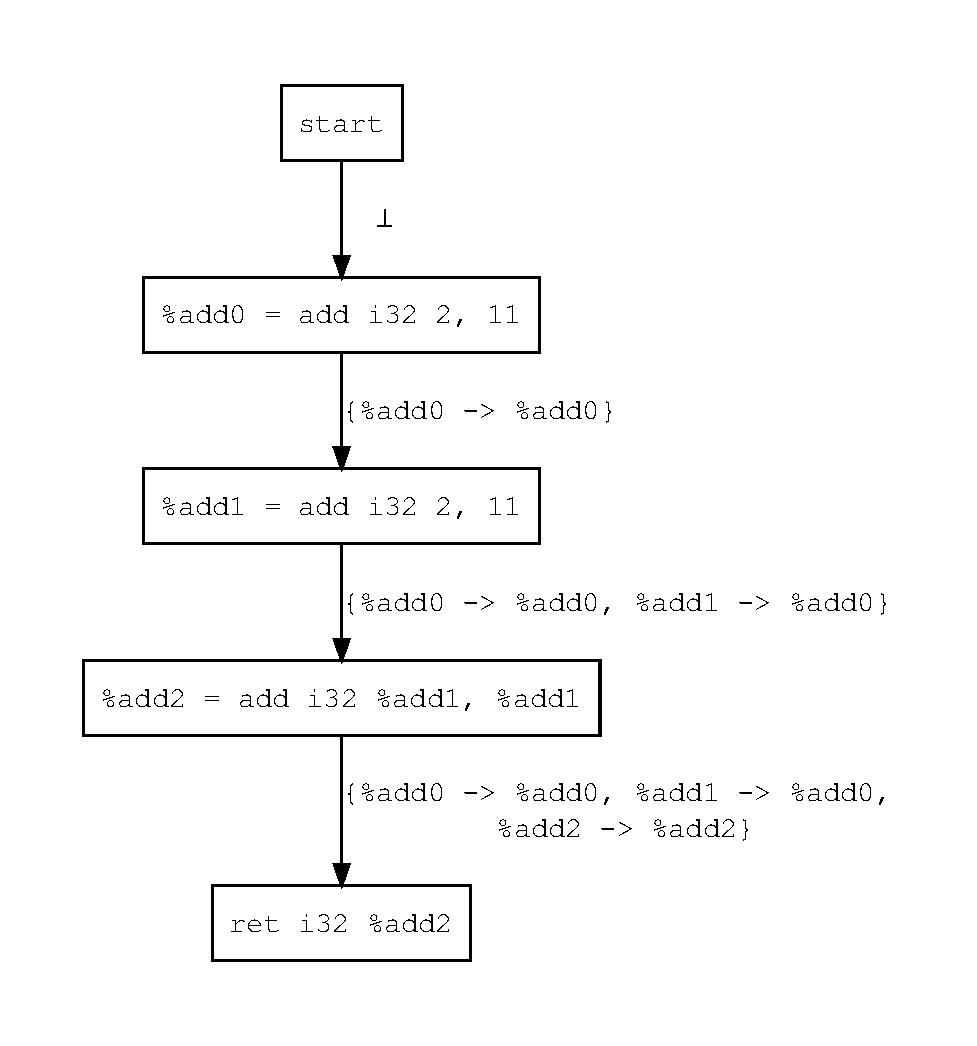
\includegraphics[scale=.4]{figures/cse/straight-line/can-do.pdf}
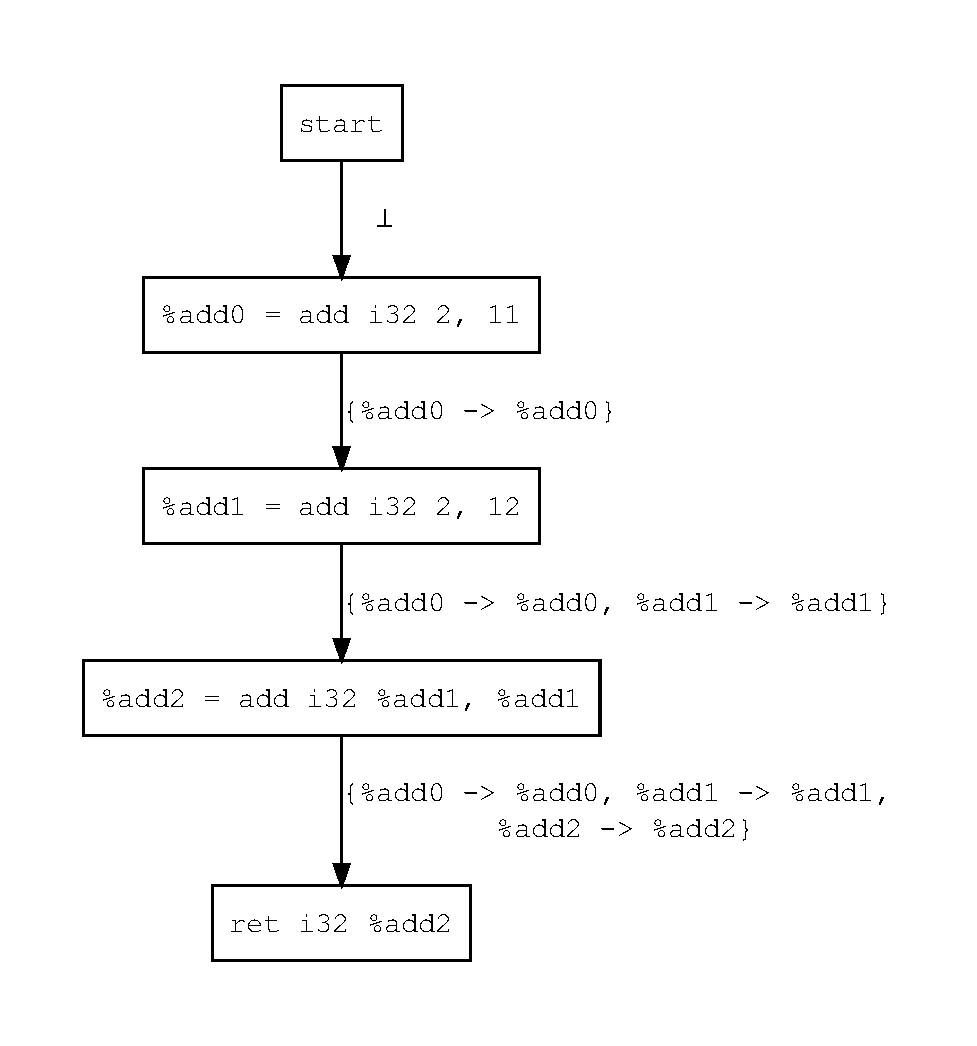
\includegraphics[scale=.4]{figures/cse/straight-line/no-do.pdf}
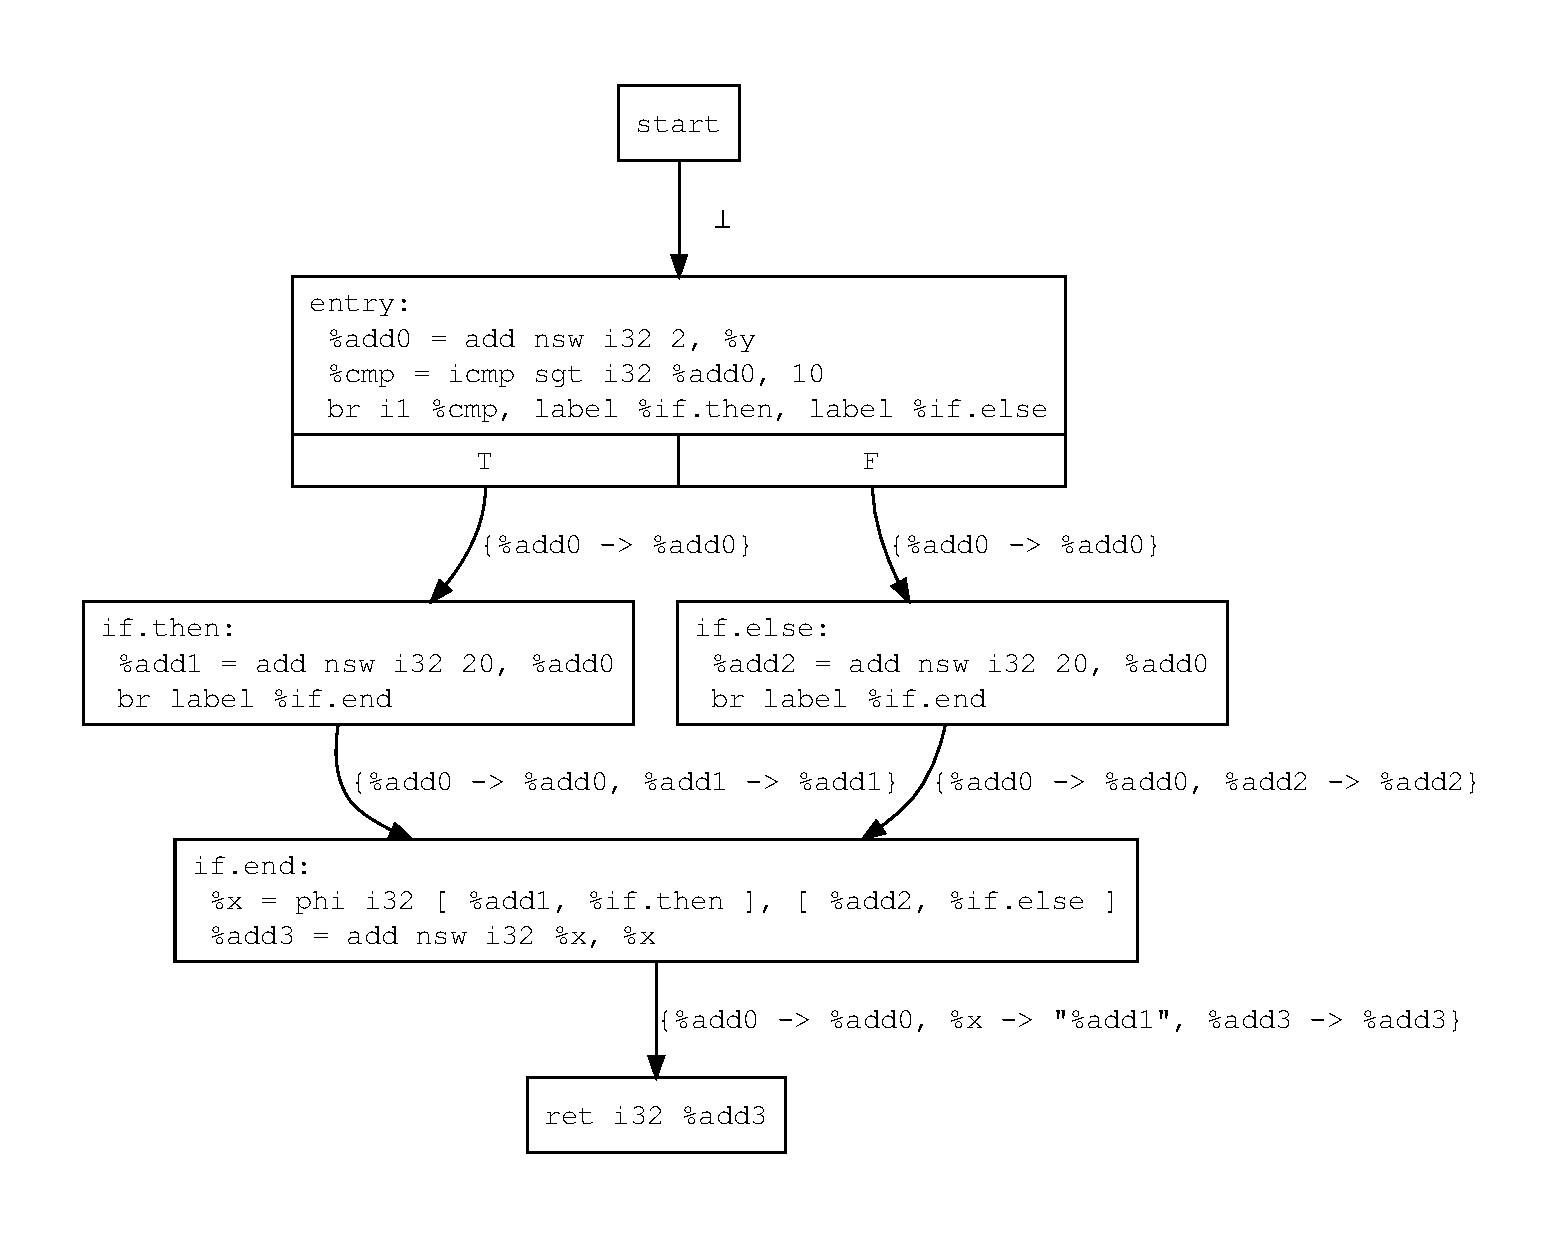
\includegraphics[scale=.4]{figures/cse/branch/can-do-cse.pdf}
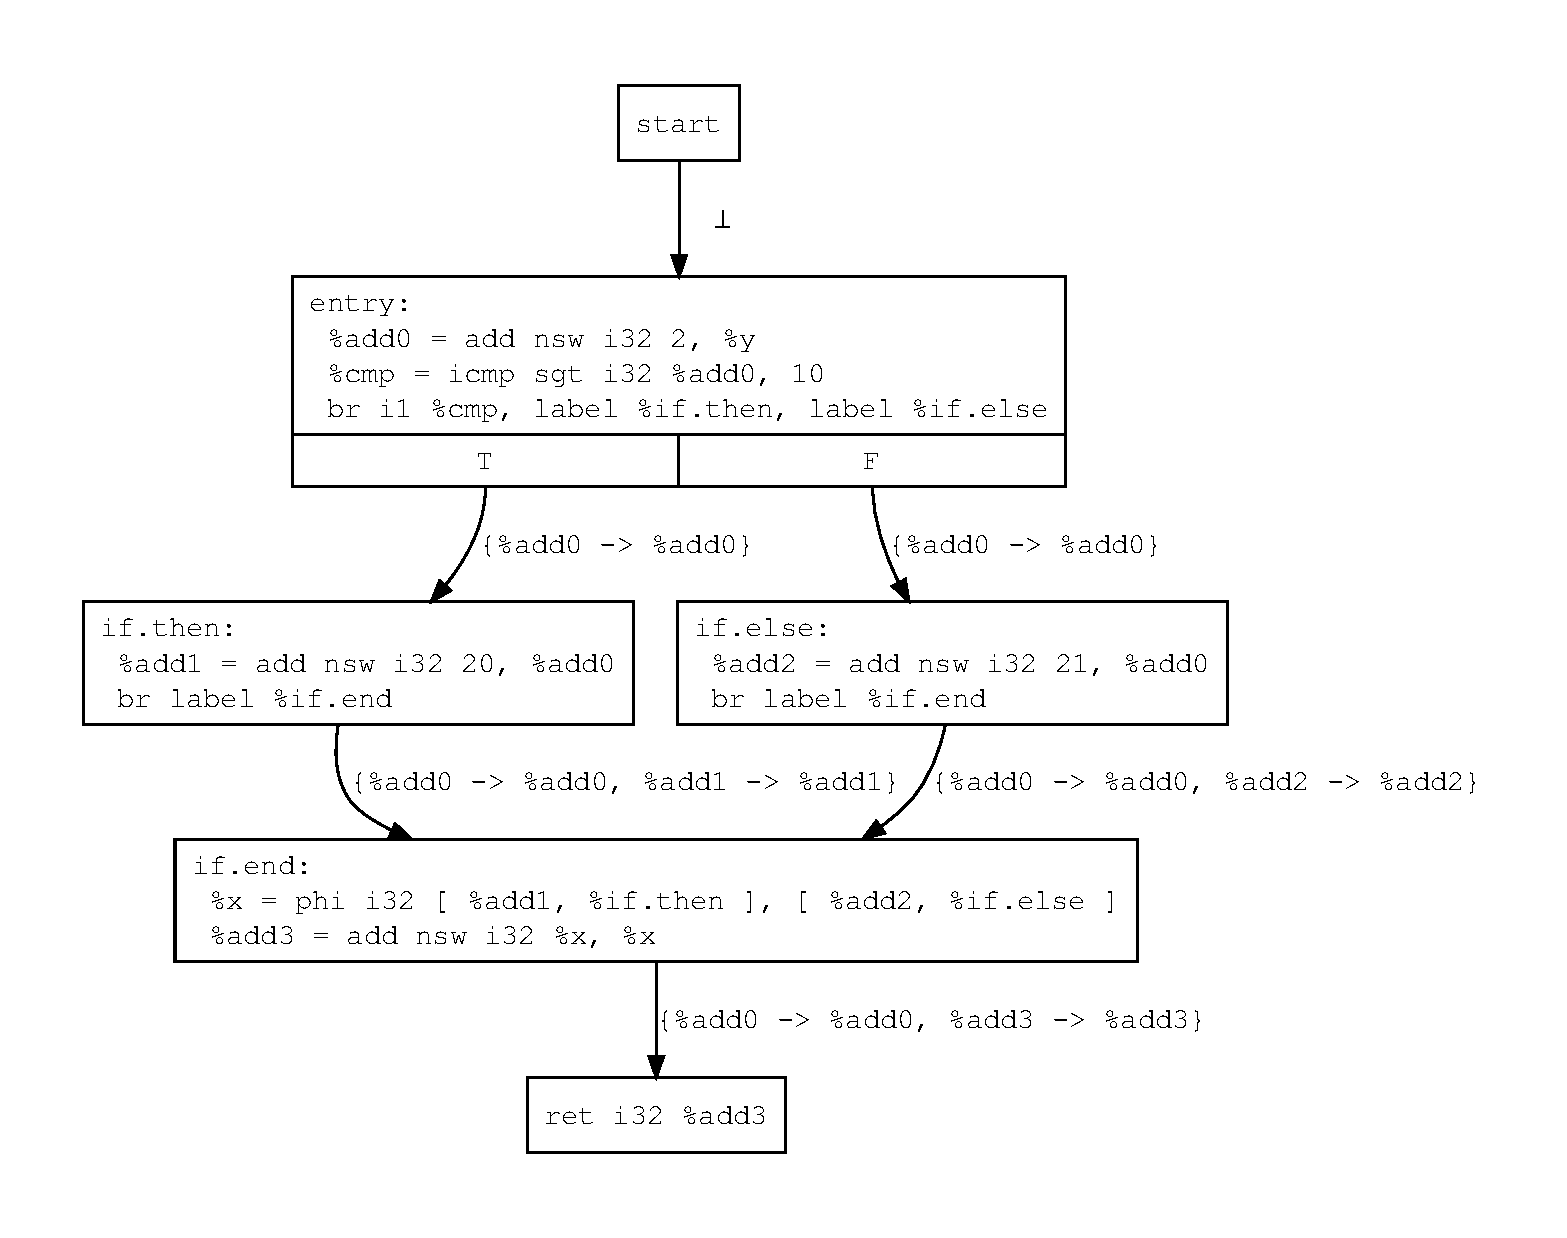
\includegraphics[scale=.4]{figures/cse/branch/no-do.pdf}

\subsection{Range Analysis}
\subsection{Intra-Procedural Pointer Analysis}



\end{document}



\section{Conclusion/Challenges}
\begin{framed}
  As this project is significantly more exploratory than the first, we
  want you to tell us what you found particularly
  interesting/challenging/frustrating. What extensions to the project
  did you attempt? (for instance, did you try combining the results of
  analyses, or did you try your hand at interprocedural
  analysis?). What aspects of LLVM made it easy/hard to implement your
  design? If you could redo your project with what you know now, what
  changes would you make?
\end{framed}
Also unsure how honest to be here. Most of our challenges had to do
with counter-intuitive LLVM design and poor documentation, as well as
the unpredictability of C++ features.

\end{document}

